%%
%% Author: thompson
%% 28.10.17
%%

% Preamble
\documentclass[11pt]{article}

% Packages
\usepackage{a4wide}
\usepackage[utf8]{inputenc}
\usepackage[ngerman]{babel}
\usepackage{scrextend}      % Intending
\usepackage{graphicx}
\usepackage{enumerate}      % Fancy listing

% Document
\begin{document}

    \section{Die 802.11 Architektur}
    Das IEEE 802.11 Protokoll ist ein Netzwerkzugangs-Protokoll welches die Konnektivität zwischen verschiedenen
    WLan-Geräten und Brücken sowie strukturierten, verkabelten Infrastrukturen sicherstellt.
    Man ermöglicht den mobilen Zugriff der User in jeder Räumlichkeit der betreffenden Gebäude - egal wo er oder sie
    sich gerade befinden. Auch verhelfen "Hot Spots" eine Erweiterung dieses Netzwerkes.

    \subsection{Logische Architektur}
    Die logische Architektur des 802.11 besteht aus mehreren Komponenten:\\
    \begin{addmargin}[1em]{1em}
        $\diamond$ (Wireless) Station (STA)\\
        Die Station ermöglicht die verbindungslose Konnektivität zum Netzwerk. Dies kann sowohl Server
        als auch Gerät eines Klienten sein.\\
        $\diamond$ (Wireless) Access Point (WAP oder AP)\\
        Der Access Point fungiert als Brücke zwischen STAs und dem gesamten Internet. Es ist quasi der jeweilige Router.\\
        $\diamond$ Independent Basic Service Set (IBSS)
        Das IBSS besteht aus mindestens 2 STAs ohne Distribution System. Auch 'Ad Hoc Wireless Network'. Verbinden sich
        beispielsweise 2 Geräte mittels Server-Client-Configuration, so verbindet sich Gerät A mit Gerät B,
        ohne Zwischenstation.\\
        $\diamond$ Basic Service Set (BSS)
        Das BSS besteht aus einem einzelnem AP, welcher mehrere STAs stützt.
        Alle STAs innerhalb eines BSS kommunizieren mittels AP und der AP überbrückt die Verbindung zum DB und damit dem
        gesamten, gebäudeinternen Netzwerk.\\
        $\diamond$ Extended Service Set (ESS)
        Ein ESS ist die Gesamtheit eines kompletten Subnetworks.
        Es ist beispielsweise ein Set aus 2 oder mehreren APs im selben Netzwerk, an welchen die STAs hängen.\\
        $\diamond$ Distribution System (DS)
        Das DS ist die Gesamtheit aller AP.
        Es erlaubt das Roaming der STAs zwischen APs.\\
    \end{addmargin}

    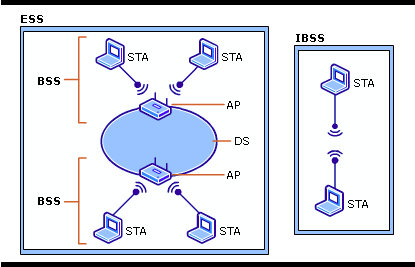
\includegraphics[width=\textwidth]{802-11_Architecture.png}
    \footnote[1{\emph{\small{Graphical Layout of the 802.11 Architecture}}}]{Source: https://i-technet.sec.s-msft.com/dynimg/IC196384.gif}

    Es gilt dabei zu beachten: Die Operationsmodi sind bei IBSS und ESS grundsätzlich unterschiedlich.

    \subsubsection{802.11 Infrastrukturmodus}
    Der Infrastrukturmodus beschreibt den Operationsmodus innerhalb des gesamten Subnets.
    Prinzipiell gibt es mindestens einen AP und einen STA, kurzum ein ESS. Der weitere Verbindungslauf wird entsprechend
    aufgerufener Ressource via AP und/oder DS geregelt.

    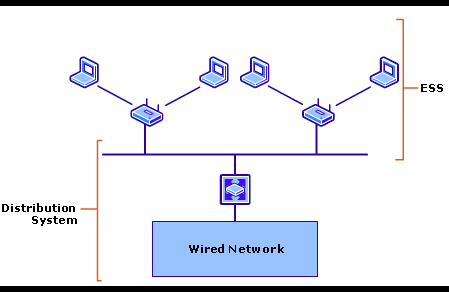
\includegraphics[width=\textwidth]{802-11_Infrastrukturmodus.png}

    \subsubsection{802.11 Ad Hoc Modus}
    \begin{minipage}{0.7\textwidth}     % Leftside :: Text using 70% of standard textwidth
        Der Ad Hoc Modus beschreibt die direkte Verbindung mehrerer STAs ohne Zwischenstationen.
        Es verläuft also ein direkter Datenverkehr zwischen mehreren Medien.
    \end{minipage}
    \begin{minipage}{0.3\textwidth}     % Rightside :: Picture using 30% of standard textwidth
        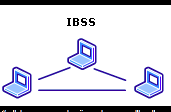
\includegraphics[width=\linewidth]{802-11_AdHoc.png}
    \end{minipage}

    \subsection{Protokolle}
    \begin{enumerate}[$\diamond$]
        \item 802.11: IEEE Norm; spezifiziert Physical Layer \& MAC
        \item 802.1X: IEEE Norm; definiert Port-basierte Zugangskontrolle
        \item EAPOL: Extensible Authentication protocol over Lan: Point-to-Point-Protocol für LANs
        \item WEP: Wired Equivalent Privacy: Dekryption zwischen WLan Nodes.
        \item WPA: Wi-Fi Protected Access: Data Enkryption \& Netzwerkauthentifizierung
    \end{enumerate}

    \subsubsection{802.11 Protokoll}

\end{document}